\chapter{Languages}

While we may think that computers are just machines, there is an incredible work behind that aims to make some kind of language that computers can understand. It is well renewed that computers act depending on streams of binary code, but that same stream of binary code can be considered as a language, something that the computers "speak" and "think" with. Let's define more in detail this "computers' language".

\begin{definition}{Alphabeth and Strings}
    An \textbf{alphabet} $\Sigma$ is a \textbf{non-empty}, \textbf{finite set}, which contains elements called \textbf{symbols} (or \textbf{characters}). For instance, the following two sets are considered alphabets:
    \begin{itemize}
        \item $\quad \Sigma = \{0, \; 1\}$
        \item $\quad \Sigma = \{a, \; b, \; c, \; \dots, \; x, \; y, \; z \}$
    \end{itemize}
    
    \noindent A \textbf{string} $w$ over an alphabet $\Sigma$ is a \textbf{sequence of symbols}, all belonging to $\Sigma$, which are all written one after the other and aren't separated by other symbols
\end{definition}

\noindent Strings also have different properties, such as a \textbf{length}, a \textbf{reverse} and the possibility to include one or more \textbf{substrings}:
\begin{itemize}
    \item \textbf{Length}: defined as $|w|$, it denotes the \textbf{number of symbols} contained within $w$. If a string has length $0$, then such string is called \textbf{empty string}, and is denoted with $\epsilon$;
    \item \textbf{Reverse}: defined as $w^R$, the reverse is a string which contains all the symbols of $w$ in the reverse order;
    \item \textbf{Substring}: we say that a string $z$ is a substring of $w$ if $z$ appears consecutively within $w$.
\end{itemize}

\begin{example}
    For instance, the string $w = 00101$ has a length of $5$, its reverse is $w^R = 10100$, and has, as possible substrings the following: $001, 10, \epsilon$. Its alphabet is $\Sigma = \{0, \; 1\}$
\end{example}

\noindent When we have two strings $x$ and $y$, we can \textbf{concatenate} them by appending $y$ at the end of $x$. The result is denoted as $xy$. Clearly, the length of the concatenated string is equal to the sum of the length of the two strings ($|xy| = |x| + |y|$). A specific notation $x^k$ denotes the concatenation of string $x$ with itself for $k$ times. So, if $x$ was for instance "$01$", then we would have that
\[ x^0 = \epsilon \quad \quad x^1 = 01 \quad \quad x^2 = 0101 \quad \quad x^3 = 010101 \quad \text{and so on...} \]

\noindent By combining the definitions of concatenation and substring, we can define properly what a \textbf{prefix} and \textbf{suffix} is:
\begin{itemize}
    \item \textbf{Prefix}: we say that a string $x$ is a prefix of a string $z$ if there exists a string $y$ such that $z = xy$. Moreover, we say that $x$ is a \textbf{proper prefix} of $z$ if, additionally, $x \neq z$, so if $y \neq \epsilon$;
    \item \textbf{Suffix}: we say that a string $x$ is a suffix of a string $z$ if there exists a string $y$ such that $z = yx$. Moreover, we say that $x$ is a \textbf{proper suffix} of $z$ if, additionally, $x \neq z$, so if $y \neq \epsilon$.
\end{itemize}

\noindent Given these tools, we can now define what a language is:

\begin{definition}{Language}
    A \textbf{language} is a \textbf{set of strings}. It is also defined as \textbf{prefix-free} if no member is a proper prefix of any other member
\end{definition}

\noindent Languages can follow an order. There are different types of orders, one of which is the \textbf{lexicographic order}, which is defined by the order of the alphabet; we can think of it as the familiar dictionary order. Another order is the \textbf{shortlex order} (or \textbf{string order}), which is the same of the lexicographic order with the exception that shorter strings precede longer strings.

\section{Deterministic Finite Automata (DFA)}

We know that sometimes circuits can use the output from a given combination of inputs as input for the next output. In that case, we talk about circuits with states, or more specifically, we talk about \textbf{automata}.

\begin{definition}{Deterministic Finite Automaton (DFA)}
    We define a \textbf{finite automaton} as a tuple of 5 elements $(Q, \; \Sigma, \; \delta, \; q_{0}, \; F)$, where:
    \begin{itemize}
        \item $Q$ is a finite set, denoting the \textbf{states} that the automaton can reach;
        \item $\Sigma$ is a finite set, denoting the \textbf{alphabet} of the automaton;
        \item $\delta$ is a function, called \textbf{transition function}, which given $Q$ and $\Sigma$ returns the set of next states $Q'$;
        \[ \delta \; : \; Q \times \Sigma \longmapsto Q'  \]
        \item $q_{0} \in Q$ is a state, and denotes the \textbf{starting state} of the automaton;
        \item $F \subseteq Q$ is a finite set, denoting the set of \textbf{accepted states} (or \textbf{final states}). An accepted state tells the automata if a string can be accepted or not.
    \end{itemize}
\end{definition}

\noindent Let's make an example:

\begin{example}
    Consider the following tuple: 
    \[ (\{ q_{1}, \; q_{2}, \; q_{3} \}, \{ 0, \; 1 \}, \delta, \; q_{1}, \; q_{2}) \]
    
    \noindent It denotes that we have 3 possible states $\{ q_{1}, \; q_{2}, \; q_{3} \}$, the alphabet is made of 2 symbols, $\{ 0, \; 1 \}$, the starting state is $q_{1}$, the final state is $q_{2}$ and the transition function is $\delta$. Such transition function could be the following: 
    \begin{center}
        \begin{tabular}{c|c c}
            & 0 & 1 \\
            \hline
            $q_{1}$ & $q_{1}$ & $q_{2}$ \\
            $q_{2}$ & $q_{3}$ & $q_{2}$ \\
            $q_{3}$ & $q_{2}$ & $q_{2}$
        \end{tabular}
    \end{center}
    
    \noindent We can represent it visually as follows:
    \begin{center}
        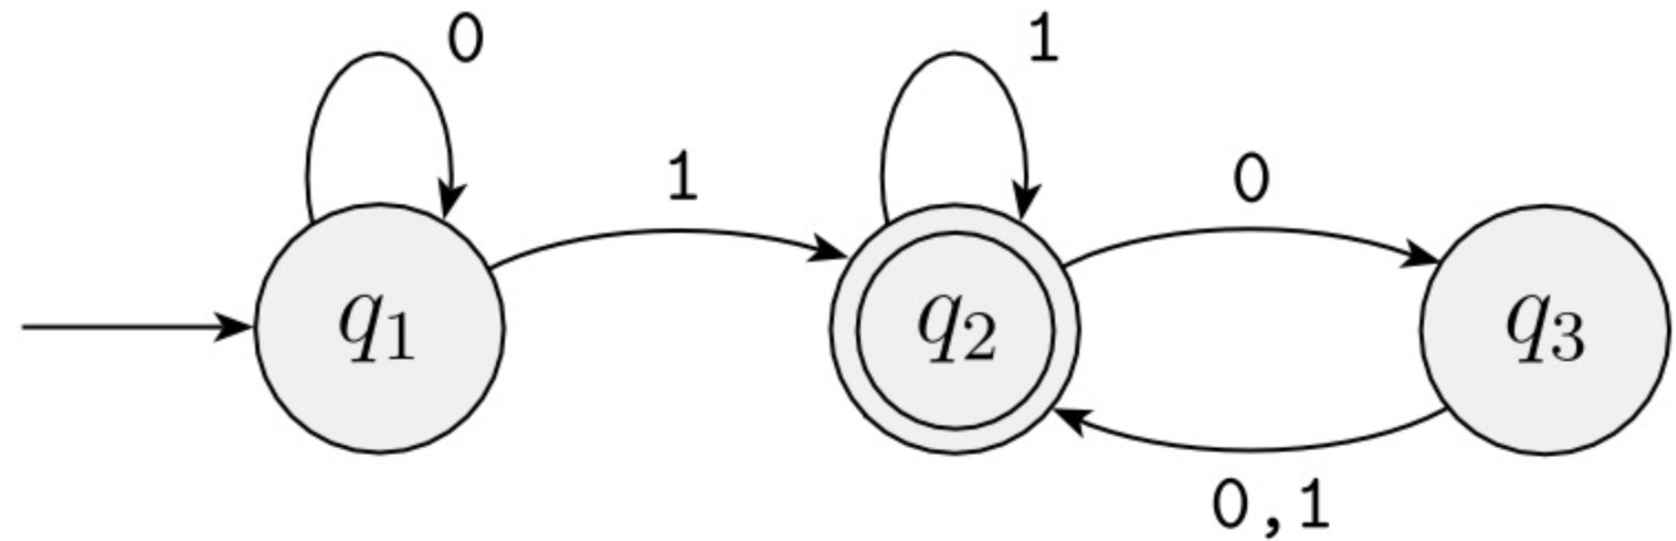
\includegraphics[scale = 0.25]{imgs/001.png}
    \end{center}
\end{example}

\noindent Automata change states depending on the string that they receive in input. So when a string $x$ is given to the automaton, it goes through the string symbol by symbol, and changes states depending on the input characters read and the result of the transition function. If, after reading the whole string, the automaton arrives at a final input, then we say that it \textbf{accepts} the string, otherwise it \textbf{rejects} it.

\begin{definition}{Language of an automaton and Regular Language}
    The \textbf{language of an automaton} $M$, denoted as $L(M)$, is the \textbf{set} of all those \textbf{input strings} which make the automaton \textbf{go} from the starting state \textbf{to} a \textbf{final state}.
    \\\\
    \noindent More specifically: given an automaton $M = (Q, \; \Sigma, \; \delta, \; q_{0}, \; F)$ and let $w$ be a string of $n$ symbols where $w_i$ denotes the $i^\text{th}$ symbol of the string; let also that
    \[ \forall \; w_{i} \in w, \text{ then } w_{i} \in \Sigma \]
    
    \noindent Then, we say that $M$ accepts $w$ if there exists a set of states $r = \{ r_{0}, \; r_{1}, \; \dots, \; r_{n} \} \in Q$ which respects all the following three conditions:
    \begin{itemize}
        \item $r_0 = q_0$: the first state of $r$ must coincide with the initial state;
        \item $\delta(r_{i}, \; w_{i + 1}) = r_{i + 1}, \; \forall  i \in [0, \; 1, \; \dots, \; n-1]$: each character must lead to a transition of state;
        \item $r_{n} \in F$: the final state in $r$ should be in $F$.
    \end{itemize}
    
    \noindent $M$ recognizes a language $A$ If
    \[ A = \{ w \; | \; M \text{ accepts } w \} \]

    \noindent A \textbf{language} $L$ is said to be \textbf{regular} if there exists a finite automaton $M$ which accepts $L$
\end{definition}

\noindent Note that it's possible for an automaton to have that $q_{0} \in F$.

\section{Non-Deterministic Finite Automata (NFA)}

With DFA, we always knew that, given a current state $q_i$ and a character $w_i \in \Sigma$, then we would \textbf{always know} what the \textbf{next state} would be. There is another type of automata which breaks this deterministic rule, and is called \textbf{non-deterministic finite automata}.

\begin{definition}{Non-Deterministic Finite Automaton (NFA)}
    A \textbf{non-deterministic finite automaton} (\textbf{NFA}) is an automaton denoted by a tuple of 5 elements $(Q, \; \Sigma, \; \delta, \; q_{0}, \; F)$ where:
    \begin{itemize}
        \item $Q$ is a finite set of \textbf{states} that the automaton can reach;
        \item $\Sigma$ denotes a finite \textbf{alphabet} recognized by the automaton;
        \item $\delta$ is the \textbf{transition function}, which given $Q$ and $\Sigma_\epsilon$ returns the \textbf{power set} of $Q$ (denoted by $\mathcal{P}(Q)$);
        \[ \delta \; : \; Q \times \Sigma_\epsilon \longmapsto \mathcal{P}(Q) \]

        \item $q_{0} \in Q$ is the \textbf{starting state} of the automaton;
        \item $F \subseteq Q$ is the set of \textbf{accepted states}.
    \end{itemize}

    \noindent The power set $\mathcal{P}(Q)$ of a set $Q$ is the set of all subsets of $Q$, for any $Q$; the alphabet denoted with $\Sigma_\epsilon$ is equal to $\Sigma \cup \{ \epsilon \}$.
\end{definition}

